
\section{Experiment 2}


In Experiment 1, perceptual similarity drove participants' mouse movements
early in reasoning,
with conceptual knowledge being drawn on later in the process,
and in some cases overriding these perceptual cues.
In Experiment 2, I attempted to replicate these finding
using artificial categories --- a kind of animal, and a kind of robot ---
that participants learned in the laboratory.
I also manipulated, between participants,
the nature of the properties to be reasoned about,
to be either \emph{specific properties}, saliently related to the two categories ---
a robot having batteries, or an animal sleeping at night, for example ---
or fictional \emph{generic properties} --- such as being able to make a ``zevy sound''.
\citet{Gelman2013c} showed that children reasoning about specific properties
were more likely to draw on conceptual knowledge,
presumably as such properties make this knowledge more salient or accessible.
Here, this manipulation provides a window into how
perceptual cues and structured representations interact during this task.

\subsection{Method}

\subsubsection{Participants}

Forty eight participants completed the experiment for course credit.

\subsubsection{Stimuli \& Procedure}

Stimuli were adapted from drawings by \citet{LaRiccia2005}
used by \citet{Sussman2014},
and consisted of cartoon pictures of different kinds of creatures.
I created two categories:
animals called ``Flurps'',
and robots called ``Floobits''.
There were four possible body shapes,
and four possible colourations,
and each body shape and colouration was possible for both Flurps and Floobits
(Figure~\ref{fig:artificial},
see also Appendix~\ref{appendix:exp2_stimuli}).

Participants were again presented with a framing story about Mark,
who had just moved to Elbee,
but this time told that Mark was learning about
different kinds of things found outdoors there.
Two kinds of thing found in Elbee were presented,
animals called ``Flurps'', and robots called ``Floobits'',
designed to closely resemble Flurps.
Participants were told that both Flurps and Floobits
had different body types
and came in different colourations,
with the same body types and colourations found in both categories.
They were also informed that Flurps and Floobits could be
differentiated by looking at their heads:
Flurps had animal heads, with tentacles on top,
while Floobits had robotic heads
(see Figure~\ref{fig:artificial}).

After these instructions, participants completed eight categorisation trials,
with feedback,
in which they were presented with four Flurps, and four Floobits,
in a random order, and asked to categorise each.
These were intended to emphasise the distinction between the categories.
% \aside{I made a coding mistake here - I have each participants' response,
%   but not what stimulus they were responding to, so I can't
%   know they were accurate here. I'm pretty sure they understood the categories
%   though, both because reasoning performance was good,
%   and because all but 2 participants selected
%   one response on half the categorisation trials
%   and the other on the rest, like they would if categorising perfectly}
After the categorisation trials,
participants were told that for the final part of the experiment
they would be told a fact about one Flurp or Floobit,
and asked to decide which of two others
this fact was most likely to also be true for.
They were then presented with the sixteen induction trials, in random order.
Half of the participants reasoning about \emph{generic} properties
that were unrelated to the two categories
(i.e. ``This one can make a zevy sound'').
The remainder reasoned about \emph{informative} properties,
so that Flurps were presented with properties specific to animals
(``This one has a mummy''),
while Floobits were presented with robot-specific properties
(``This one has batteries inside'').
The full list of properties used can be found in
Appendix~\ref{appendix:exp2_properties}.

There were sixteen induction trials,
eight with Flurps as bases,
and eight with Floobits,
and the response options always consisted of
one Flurp and one Floobit.
Half of these were control trials,
in that the response entity belonging to
the same category as the base (the correct response)
was perceptually identical to the base,
having the same body type and colouration,
while the other, foil response entity was perceptually different,
with a different body type and colouration.
The remainder were conflict trials (Figure~\ref{fig:artificial}),
where the correct response was perceptually different from the base,
and the foil response was perceptually similar.

\begin{figure}[ht]
  \centering
  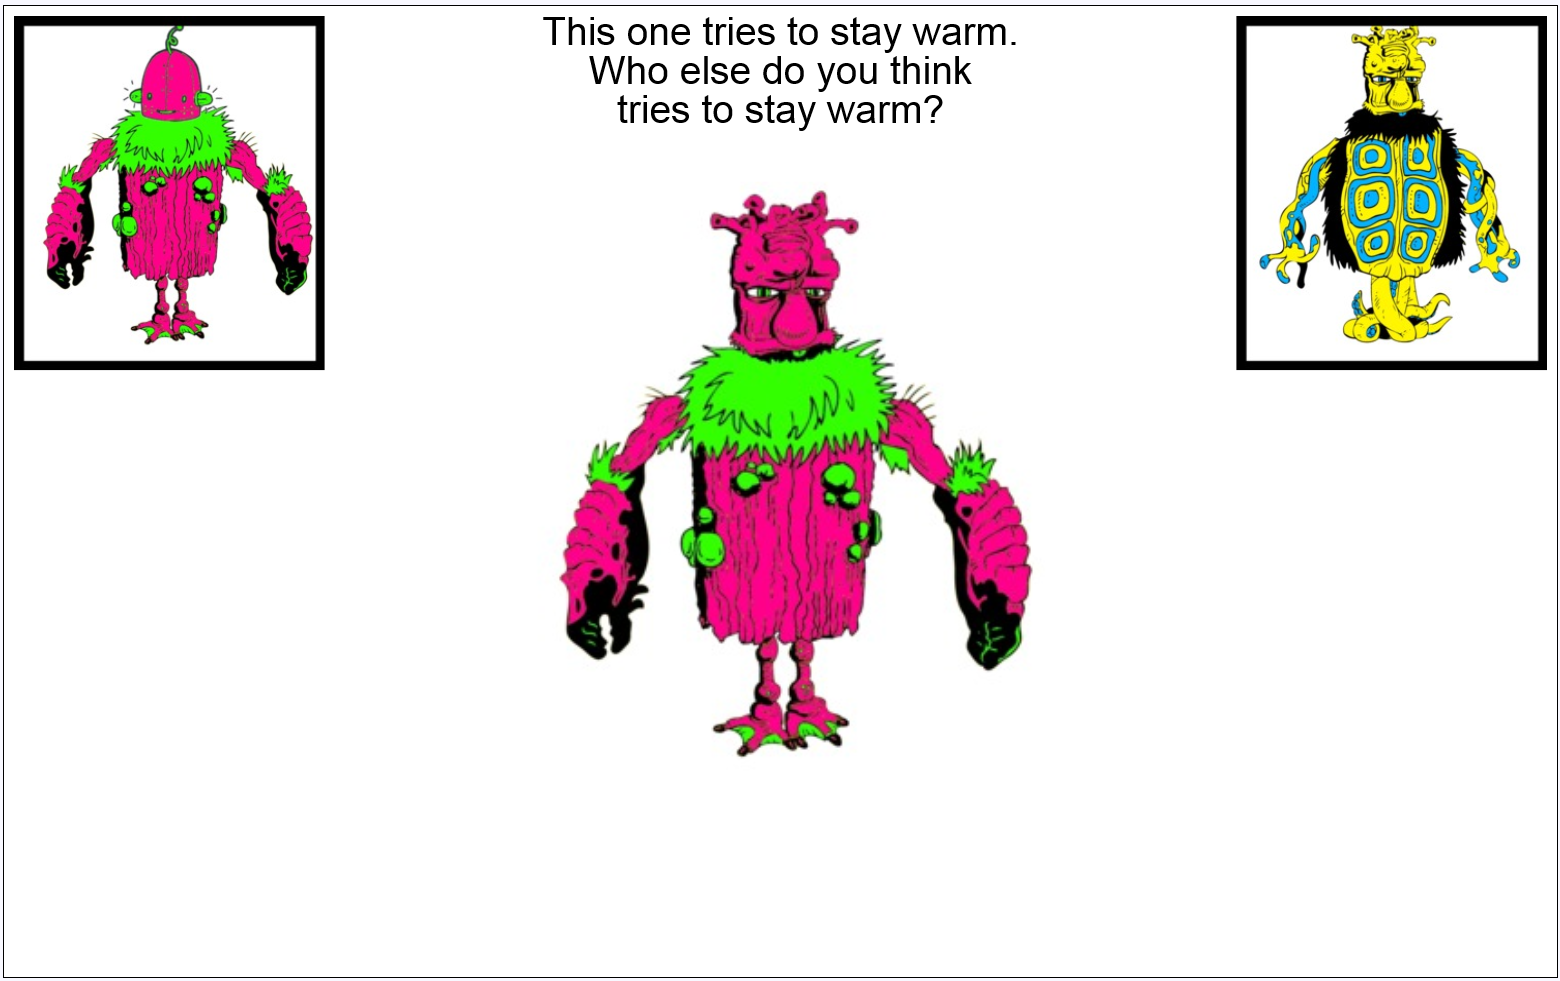
\includegraphics[width=\figurewidth]{imgs/artificial_screenshot.png}
  \caption[Screen shot from Experiment 2.]{
    A trial from Experiment 2.
    Participants were told that the \emph{Flurp} (centre)
    tries to stay warm, and asked to decide
    which of the other two things shown,
    the \emph{Floobit} on the left, or the Flurp on the right,
    also tries to stay warm.
    This is a conflict trial:
    the Floobit has the same colouration and body type as the base,
    but its robotic head identifies it as belonging to a different category.
    \label{fig:artificial}
  }
\end{figure}


